
%% bare_jrnl.tex
%% V1.3
%% 2007/01/11
%% by Michael Shell
%% see http://www.michaelshell.org/
%% for current contact information.
%%
%% This is a skeleton file demonstrating the use of IEEEtran.cls
%% (requires IEEEtran.cls version 1.7 or later) with an IEEE journal paper.
%%
%% Support sites:
%% http://www.michaelshell.org/tex/ieeetran/
%% http://www.ctan.org/tex-archive/macros/latex/contrib/IEEEtran/
%% and
%% http://www.ieee.org/



% *** Authors should verify (and, if needed, correct) their LaTeX system  ***
% *** with the testflow diagnostic prior to trusting their LaTeX platform ***
% *** with production work. IEEE's font choices can trigger bugs that do  ***
% *** not appear when using other class files.                            ***
% The testflow support page is at:
% http://www.michaelshell.org/tex/testflow/


%%*************************************************************************
%% Legal Notice:
%% This code is offered as-is without any warranty either expressed or
%% implied; without even the implied warranty of MERCHANTABILITY or
%% FITNESS FOR A PARTICULAR PURPOSE! 
%% User assumes all risk.
%% In no event shall IEEE or any contributor to this code be liable for
%% any damages or losses, including, but not limited to, incidental,
%% consequential, or any other damages, resulting from the use or misuse
%% of any information contained here.
%%
%% All comments are the opinions of their respective authors and are not
%% necessarily endorsed by the IEEE.
%%
%% This work is distributed under the LaTeX Project Public License (LPPL)
%% ( http://www.latex-project.org/ ) version 1.3, and may be freely used,
%% distributed and modified. A copy of the LPPL, version 1.3, is included
%% in the base LaTeX documentation of all distributions of LaTeX released
%% 2003/12/01 or later.
%% Retain all contribution notices and credits.
%% ** Modified files should be clearly indicated as such, including  **
%% ** renaming them and changing author support contact information. **
%%
%% File list of work: IEEEtran.cls, IEEEtran_HOWTO.pdf, bare_adv.tex,
%%                    bare_conf.tex, bare_jrnl.tex, bare_jrnl_compsoc.tex
%%*************************************************************************

% Note that the a4paper option is mainly intended so that authors in
% countries using A4 can easily print to A4 and see how their papers will
% look in print - the typesetting of the document will not typically be
% affected with changes in paper size (but the bottom and side margins will).
% Use the testflow package mentioned above to verify correct handling of
% both paper sizes by the user's LaTeX system.
%
% Also note that the "draftcls" or "draftclsnofoot", not "draft", option
% should be used if it is desired that the figures are to be displayed in
% draft mode.
%
\documentclass[journal]{IEEEtran}
%
% If IEEEtran.cls has not been installed into the LaTeX system files,
% manually specify the path to it like:
% \documentclass[journal]{../sty/IEEEtran}





% Some very useful LaTeX packages include:
% (uncomment the ones you want to load)


% *** MISC UTILITY PACKAGES ***
%
%\usepackage{ifpdf}
% Heiko Oberdiek's ifpdf.sty is very useful if you need conditional
% compilation based on whether the output is pdf or dvi.
% usage:
% \ifpdf
%   % pdf code
% \else
%   % dvi code
% \fi
% The latest version of ifpdf.sty can be obtained from:
% http://www.ctan.org/tex-archive/macros/latex/contrib/oberdiek/
% Also, note that IEEEtran.cls V1.7 and later provides a builtin
% \ifCLASSINFOpdf conditional that works the same way.
% When switching from latex to pdflatex and vice-versa, the compiler may
% have to be run twice to clear warning/error messages.






% *** CITATION PACKAGES ***
%
\usepackage{cite}
\usepackage{times,graphics,epsfig, enumerate, pifont, amsfonts, amssymb, rotating}

% cite.sty was written by Donald Arseneau
% V1.6 and later of IEEEtran pre-defines the format of the cite.sty package
% \cite{} output to follow that of IEEE. Loading the cite package will
% result in citation numbers being automatically sorted and properly
% "compressed/ranged". e.g., [1], [9], [2], [7], [5], [6] without using
% cite.sty will become [1], [2], [5]--[7], [9] using cite.sty. cite.sty's
% \cite will automatically add leading space, if needed. Use cite.sty's
% noadjust option (cite.sty V3.8 and later) if you want to turn this off.
% cite.sty is already installed on most LaTeX systems. Be sure and use
% version 4.0 (2003-05-27) and later if using hyperref.sty. cite.sty does
% not currently provide for hyperlinked citations.
% The latest version can be obtained at:
% http://www.ctan.org/tex-archive/macros/latex/contrib/cite/
% The documentation is contained in the cite.sty file itself.






% *** GRAPHICS RELATED PACKAGES ***
%
\ifCLASSINFOpdf
  % \usepackage[pdftex]{graphicx}
  % declare the path(s) where your graphic files are
  % \graphicspath{{../pdf/}{../jpeg/}}
  % and their extensions so you won't have to specify these with
  % every instance of \includegraphics
  % \DeclareGraphicsExtensions{.pdf,.jpeg,.png}
\else
  % or other class option (dvipsone, dvipdf, if not using dvips). graphicx
  % will default to the driver specified in the system graphics.cfg if no
  % driver is specified.
  % \usepackage[dvips]{graphicx}
  % declare the path(s) where your graphic files are
  % \graphicspath{{../eps/}}
  % and their extensions so you won't have to specify these with
  % every instance of \includegraphics
  % \DeclareGraphicsExtensions{.eps}
\fi
% graphicx was written by David Carlisle and Sebastian Rahtz. It is
% required if you want graphics, photos, etc. graphicx.sty is already
% installed on most LaTeX systems. The latest version and documentation can
% be obtained at: 
% http://www.ctan.org/tex-archive/macros/latex/required/graphics/
% Another good source of documentation is "Using Imported Graphics in
% LaTeX2e" by Keith Reckdahl which can be found as epslatex.ps or
% epslatex.pdf at: http://www.ctan.org/tex-archive/info/
%
% latex, and pdflatex in dvi mode, support graphics in encapsulated
% postscript (.eps) format. pdflatex in pdf mode supports graphics
% in .pdf, .jpeg, .png and .mps (metapost) formats. Users should ensure
% that all non-photo figures use a vector format (.eps, .pdf, .mps) and
% not a bitmapped formats (.jpeg, .png). IEEE frowns on bitmapped formats
% which can result in "jaggedy"/blurry rendering of lines and letters as
% well as large increases in file sizes.
%
% You can find documentation about the pdfTeX application at:
% http://www.tug.org/applications/pdftex





% *** MATH PACKAGES ***
%
%\usepackage[cmex10]{amsmath}
% A popular package from the American Mathematical Society that provides
% many useful and powerful commands for dealing with mathematics. If using
% it, be sure to load this package with the cmex10 option to ensure that
% only type 1 fonts will utilized at all point sizes. Without this option,
% it is possible that some math symbols, particularly those within
% footnotes, will be rendered in bitmap form which will result in a
% document that can not be IEEE Xplore compliant!
%
% Also, note that the amsmath package sets \interdisplaylinepenalty to 10000
% thus preventing page breaks from occurring within multiline equations. Use:
%\interdisplaylinepenalty=2500
% after loading amsmath to restore such page breaks as IEEEtran.cls normally
% does. amsmath.sty is already installed on most LaTeX systems. The latest
% version and documentation can be obtained at:
% http://www.ctan.org/tex-archive/macros/latex/required/amslatex/math/





% *** SPECIALIZED LIST PACKAGES ***
%
%\usepackage{algorithmic}
% algorithmic.sty was written by Peter Williams and Rogerio Brito.
% This package provides an algorithmic environment fo describing algorithms.
% You can use the algorithmic environment in-text or within a figure
% environment to provide for a floating algorithm. Do NOT use the algorithm
% floating environment provided by algorithm.sty (by the same authors) or
% algorithm2e.sty (by Christophe Fiorio) as IEEE does not use dedicated
% algorithm float types and packages that provide these will not provide
% correct IEEE style captions. The latest version and documentation of
% algorithmic.sty can be obtained at:
% http://www.ctan.org/tex-archive/macros/latex/contrib/algorithms/
% There is also a support site at:
% http://algorithms.berlios.de/index.html
% Also of interest may be the (relatively newer and more customizable)
% algorithmicx.sty package by Szasz Janos:
% http://www.ctan.org/tex-archive/macros/latex/contrib/algorithmicx/




% *** ALIGNMENT PACKAGES ***
%
%\usepackage{array}
% Frank Mittelbach's and David Carlisle's array.sty patches and improves
% the standard LaTeX2e array and tabular environments to provide better
% appearance and additional user controls. As the default LaTeX2e table
% generation code is lacking to the point of almost being broken with
% respect to the quality of the end results, all users are strongly
% advised to use an enhanced (at the very least that provided by array.sty)
% set of table tools. array.sty is already installed on most systems. The
% latest version and documentation can be obtained at:
% http://www.ctan.org/tex-archive/macros/latex/required/tools/


%\usepackage{mdwmath}
%\usepackage{mdwtab}
% Also highly recommended is Mark Wooding's extremely powerful MDW tools,
% especially mdwmath.sty and mdwtab.sty which are used to format equations
% and tables, respectively. The MDWtools set is already installed on most
% LaTeX systems. The lastest version and documentation is available at:
% http://www.ctan.org/tex-archive/macros/latex/contrib/mdwtools/


% IEEEtran contains the IEEEeqnarray family of commands that can be used to
% generate multiline equations as well as matrices, tables, etc., of high
% quality.


%\usepackage{eqparbox}
% Also of notable interest is Scott Pakin's eqparbox package for creating
% (automatically sized) equal width boxes - aka "natural width parboxes".
% Available at:
% http://www.ctan.org/tex-archive/macros/latex/contrib/eqparbox/





% *** SUBFIGURE PACKAGES ***
%\usepackage[tight,footnotesize]{subfigure}
% subfigure.sty was written by Steven Douglas Cochran. This package makes it
% easy to put subfigures in your figures. e.g., "Figure 1a and 1b". For IEEE
% work, it is a good idea to load it with the tight package option to reduce
% the amount of white space around the subfigures. subfigure.sty is already
% installed on most LaTeX systems. The latest version and documentation can
% be obtained at:
% http://www.ctan.org/tex-archive/obsolete/macros/latex/contrib/subfigure/
% subfigure.sty has been superceeded by subfig.sty.



%\usepackage[caption=false]{caption}
%\usepackage[font=footnotesize]{subfig}
% subfig.sty, also written by Steven Douglas Cochran, is the modern
% replacement for subfigure.sty. However, subfig.sty requires and
% automatically loads Axel Sommerfeldt's caption.sty which will override
% IEEEtran.cls handling of captions and this will result in nonIEEE style
% figure/table captions. To prevent this problem, be sure and preload
% caption.sty with its "caption=false" package option. This is will preserve
% IEEEtran.cls handing of captions. Version 1.3 (2005/06/28) and later 
% (recommended due to many improvements over 1.2) of subfig.sty supports
% the caption=false option directly:
%\usepackage[caption=false,font=footnotesize]{subfig}
%
% The latest version and documentation can be obtained at:
% http://www.ctan.org/tex-archive/macros/latex/contrib/subfig/
% The latest version and documentation of caption.sty can be obtained at:
% http://www.ctan.org/tex-archive/macros/latex/contrib/caption/




% *** FLOAT PACKAGES ***
%
%\usepackage{fixltx2e}
% fixltx2e, the successor to the earlier fix2col.sty, was written by
% Frank Mittelbach and David Carlisle. This package corrects a few problems
% in the LaTeX2e kernel, the most notable of which is that in current
% LaTeX2e releases, the ordering of single and double column floats is not
% guaranteed to be preserved. Thus, an unpatched LaTeX2e can allow a
% single column figure to be placed prior to an earlier double column
% figure. The latest version and documentation can be found at:
% http://www.ctan.org/tex-archive/macros/latex/base/



%\usepackage{stfloats}
% stfloats.sty was written by Sigitas Tolusis. This package gives LaTeX2e
% the ability to do double column floats at the bottom of the page as well
% as the top. (e.g., "\begin{figure*}[!b]" is not normally possible in
% LaTeX2e). It also provides a command:
%\fnbelowfloat
% to enable the placement of footnotes below bottom floats (the standard
% LaTeX2e kernel puts them above bottom floats). This is an invasive package
% which rewrites many portions of the LaTeX2e float routines. It may not work
% with other packages that modify the LaTeX2e float routines. The latest
% version and documentation can be obtained at:
% http://www.ctan.org/tex-archive/macros/latex/contrib/sttools/
% Documentation is contained in the stfloats.sty comments as well as in the
% presfull.pdf file. Do not use the stfloats baselinefloat ability as IEEE
% does not allow \baselineskip to stretch. Authors submitting work to the
% IEEE should note that IEEE rarely uses double column equations and
% that authors should try to avoid such use. Do not be tempted to use the
% cuted.sty or midfloat.sty packages (also by Sigitas Tolusis) as IEEE does
% not format its papers in such ways.


%\ifCLASSOPTIONcaptionsoff
%  \usepackage[nomarkers]{endfloat}
% \let\MYoriglatexcaption\caption
% \renewcommand{\caption}[2][\relax]{\MYoriglatexcaption[#2]{#2}}
%\fi
% endfloat.sty was written by James Darrell McCauley and Jeff Goldberg.
% This package may be useful when used in conjunction with IEEEtran.cls'
% captionsoff option. Some IEEE journals/societies require that submissions
% have lists of figures/tables at the end of the paper and that
% figures/tables without any captions are placed on a page by themselves at
% the end of the document. If needed, the draftcls IEEEtran class option or
% \CLASSINPUTbaselinestretch interface can be used to increase the line
% spacing as well. Be sure and use the nomarkers option of endfloat to
% prevent endfloat from "marking" where the figures would have been placed
% in the text. The two hack lines of code above are a slight modification of
% that suggested by in the endfloat docs (section 8.3.1) to ensure that
% the full captions always appear in the list of figures/tables - even if
% the user used the short optional argument of \caption[]{}.
% IEEE papers do not typically make use of \caption[]'s optional argument,
% so this should not be an issue. A similar trick can be used to disable
% captions of packages such as subfig.sty that lack options to turn off
% the subcaptions:
% For subfig.sty:
% \let\MYorigsubfloat\subfloat
% \renewcommand{\subfloat}[2][\relax]{\MYorigsubfloat[]{#2}}
% For subfigure.sty:
% \let\MYorigsubfigure\subfigure
% \renewcommand{\subfigure}[2][\relax]{\MYorigsubfigure[]{#2}}
% However, the above trick will not work if both optional arguments of
% the \subfloat/subfig command are used. Furthermore, there needs to be a
% description of each subfigure *somewhere* and endfloat does not add
% subfigure captions to its list of figures. Thus, the best approach is to
% avoid the use of subfigure captions (many IEEE journals avoid them anyway)
% and instead reference/explain all the subfigures within the main caption.
% The latest version of endfloat.sty and its documentation can obtained at:
% http://www.ctan.org/tex-archive/macros/latex/contrib/endfloat/
%
% The IEEEtran \ifCLASSOPTIONcaptionsoff conditional can also be used
% later in the document, say, to conditionally put the References on a 
% page by themselves.





% *** PDF, URL AND HYPERLINK PACKAGES ***
%
%\usepackage{url}
% url.sty was written by Donald Arseneau. It provides better support for
% handling and breaking URLs. url.sty is already installed on most LaTeX
% systems. The latest version can be obtained at:
% http://www.ctan.org/tex-archive/macros/latex/contrib/misc/
% Read the url.sty source comments for usage information. Basically,
% \url{my_url_here}.





% *** Do not adjust lengths that control margins, column widths, etc. ***
% *** Do not use packages that alter fonts (such as pslatex).         ***
% There should be no need to do such things with IEEEtran.cls V1.6 and later.
% (Unless specifically asked to do so by the journal or conference you plan
% to submit to, of course. )


% correct bad hyphenation here
\hyphenation{op-tical net-works semi-conduc-tor}


\begin{document}
%
% paper title
% can use linebreaks \\ within to get better formatting as desired
\title{Testing .NET Code with YETI}
%
%
% author names and IEEE memberships
% note positions of commas and nonbreaking spaces ( ~ ) LaTeX will not break
% a structure at a ~ so this keeps an author's name from being broken across
% two lines.
% use \thanks{} to gain access to the first footnote area
% a separate \thanks must be used for each paragraph as LaTeX2e's \thanks
% was not built to handle multiple paragraphs
%

\author{Manuel~Oriol,\thanks{M. Oriol is with University of York.}
        Sotirios Tassis\thanks{S. Tassis was a student at University of York.}
% <-this % stops a space
%\thanks{M. Shell is with the Department
%of Electrical and Computer Engineering, Georgia Institute of Technology, Atlanta,
%GA, 30332 USA e-mail: (see http://www.michaelshell.org/contact.html).}% <-this % stops a space
%\thanks{J. Doe and J. Doe are with Anonymous University.}% <-this % stops a space
%\thanks{Manuscript received April 19, 2005; revised January 11, 2007.}
}

% note the % following the last \IEEEmembership and also \thanks - 
% these prevent an unwanted space from occurring between the last author name
% and the end of the author line. i.e., if you had this:
% 
% \author{....lastname \thanks{...} \thanks{...} }
%                     ^------------^------------^----Do not want these spaces!
%
% a space would be appended to the last name and could cause every name on that
% line to be shifted left slightly. This is one of those "LaTeX things". For
% instance, "\textbf{A} \textbf{B}" will typeset as "A B" not "AB". To get
% "AB" then you have to do: "\textbf{A}\textbf{B}"
% \thanks is no different in this regard, so shield the last } of each \thanks
% that ends a line with a % and do not let a space in before the next \thanks.
% Spaces after \IEEEmembership other than the last one are OK (and needed) as
% you are supposed to have spaces between the names. For what it is worth,
% this is a minor point as most people would not even notice if the said evil
% space somehow managed to creep in.



% The paper headers
\markboth{Journal ?,~Vol.~?, No.~?, January~?}%
{Testing .NET Code with YETI}
% The only time the second header will appear is for the odd numbered pages
% after the title page when using the twoside option.
% 
% *** Note that you probably will NOT want to include the author's ***
% *** name in the headers of peer review papers.                   ***
% You can use \ifCLASSOPTIONpeerreview for conditional compilation here if
% you desire.




% If you want to put a publisher's ID mark on the page you can do it like
% this:
%\IEEEpubid{0000--0000/00\$00.00~\copyright~2007 IEEE}
% Remember, if you use this you must call \IEEEpubidadjcol in the second
% column for its text to clear the IEEEpubid mark.



% use for special paper notices
%\IEEEspecialpapernotice{(Invited Paper)}




% make the title area
\maketitle

\begin{abstract}
Random testing is a simple technique quite effective at finding faults.
There is to date no single system that would cope with several programming languages and provide some level of reuse of code and concepts. There is also very little interaction between test engineers and the random testing platform while testing.

This article presents the York Extendible Testing Infrastructure (YETI), a random testing tool implemented in Java that allows the testing of code written in multiple programming languages (currently Java, JML and .NET). YETI provides a strong decoupling between the strategies and the actual language binding. The tool exhibits unparalleled performances with around $10^6$ calls per minute on Java code. It also benefits from a graphical user interface that allows test engineer to orient the testing process while testing. We illustrate the efficiency of such a tool  with a study testing all classes in java.lang and some classes in the well known open source project iText, a PDF document manipulation Java library.

\end{abstract}

% Note that keywords are not normally used for peerreview papers.
\begin{IEEEkeywords}
IEEEtran, journal, \LaTeX, paper, template.
\end{IEEEkeywords}






% For peer review papers, you can put extra information on the cover
% page as needed:
% \ifCLASSOPTIONpeerreview
% \begin{center} \bfseries EDICS Category: 3-BBND \end{center}
% \fi
%
% For peerreview papers, this IEEEtran command inserts a page break and
% creates the second title. It will be ignored for other modes.
\IEEEpeerreviewmaketitle

\newcommand{\subtype}{\ensuremath{\unlhd}}



\section{Introduction}\label{sec:intro}

Automated random testing is a methodology often neglected by 
programmers and software testers because it seems overly
simple. It has however advantages over other techniques because 
it is completely unbiased and allows the execution of a high number 
of calls over a short period of time.


The York Extendible Testing Infrastructure (YETI) provides a framework 
for executing random testing sessions. The main characteristics of 
YETI is that it supports multiple programming languages through a 
language-agnostic meta model. Various testing strategies apply
to all supported languages thanks to a strong decoupling between the 
strategies used and the programming language binding. 

Oracles are language-dependent. In the presence of specifications YETI checks 
inconsistencies between the code and the specifications. In the case of 
languages such as plain Java, if programmers use \texttt{assert} statements 
then violations are interpreted as failures. If programmers do not use assert 
statements a testing session with YETI is a robustness test that
considers undeclared runtime exceptions thrown as failures.

Unlike competitors, YETI also support a graphical user interface that 
allows test engineers to monitor the testing session and modify some 
of its characteristics while testing. To validate our approach we made 
one million calls at random on each class in \texttt{java.lang} where 
it discovered 45 faults. We also tested a package of iText where it 
discovered 120 faults. 


Section~\ref{sec:model} presents YETI's meta-model and its main algorithms.
Section~\ref{sec:implem} describes its current implementation.
Section~\ref{sec:evaluation} evaluates YETI.
Section~\ref{sec:rw} presents related work.
We eventually conclude in Section~\ref{sec:conc}.
\section{Model}\label{sec:model}

This section describes the meta-model used by YETI to represent programs 
and data. The actual model was previously describe in an article describing the Java 
binding of YETI~\cite{Oriol:10:YETI}, please refer to it for a complete definition of the 
model.

YETI uses four main notions: 

\begin{description}
\item{\textbf{Routines:}} A routine is a computation unit that uses variables of a given type and 
returns values of a given type:
\begin{equation}
\ensuremath{R::=(T_{1} \times...\times T_{k}) \rightarrow T_{0}}
\label{equ:routine}
\end{equation}
\item{\textbf{Types:}} A type is a collection of variables and a collection of routines that
return values�(of that type):
\begin{equation}
\ensuremath{T::=((R_{1},...,R_{k}),(V_{1},...,V_{l}))}
\label{equ:type}
\end{equation}
\item{\textbf{Variables:}} A variable is a couple between a 
label and a value:
\begin{equation}
\ensuremath{V::=(n,v)}
\label{equ:variable}
\end{equation}
\item{\textbf{Modules:}}   A module is a collection of routines:
\begin{equation}
\ensuremath{M::=(R_{1},...,R_{k})}
\label{equ:module}
\end{equation}
\end{description}  

This model is used by YETI as the backbone of any binding. Note that types can be organized 
through a subtyping relationship which imposes that all variables of a subtype are also present 
in the super type and that all types constructors of the subtype are also constructors of the 
supertype. YETI ensures that the these properties are verified.

While these definitions model a program from a high level that is not concerned with actual values
and computation, it is enough for devising strategies. As an example,  Figure~\ref{fig:rand} shows the algorithm -- in C\#-like pseudo code -- of the pure random strategy.

\begin{figure}[h]
\begin{verbatim}
M0 = .../** module to test **/
while (not endReached){
  R0=M0.getRandomRoutine();
  Vector<Variables> arguments = 
           new Vector<Variable>();
  for(T in R0.getArguments()){
   arguments.addLast(
         T.getArgumentAtRandom());
  }
  try {
    new Variable(R0.call(arguments));
  } catch (Exception e) {
    if (not 
         (e is PreconditionViolation)){
     foundBugs.add(e);
    }
  }
}
\end{verbatim}
\caption{Algorithm for the random strategy.}\label{fig:rand}
\end{figure}

What Figure~\ref{fig:rand} does not show is the generation of new variables other than through making calls.
In this example, we assume that this happens in \verb+T.getArgumentAtRandom()+. It could however be added to the algorithm without any issue.

Other strategies are however possible. For example Random+~\cite{CMOP:08:FFMTRTUR} either picks selects values in the existing pool of object, generate new ones on the fly, or take interesting values. This implies that the model should be enriched to take into account a set of interesting values in each type. In practice, this is exactly what happens, and up to now, we always managed to introduce backward compatible changes.

\section{Architecture and implementation}\label{sec:architecture}

\subsection{YETI standalone application}
YETI is an automated random testing tool for Java. 
A YETI testing session consists in a sequence of calls made to methods at
random using arguments generated at random. 
The oracle for the tests are either contracts --�when available -- or runtime 
exceptions/failures.

When a failure is detected the logs of the testing session are minimised to 
produce test cases that reproduce the failure. Such unit tests can then be stored and 
be executed later by a unit test framework.

YETI is usually launched on the command-line. A typical call to YETI is:
{\small
\begin{verbatim}
java yeti.Yeti -Java -yetiPath=. 
          -time=10mn -randomPlus
          -testModules=String:StringBuilder 
\end{verbatim}
}

The options used on this command-line have the following meaning: \texttt{-Java} 
indicates that the tested program is in Java, \texttt{-yetiPath=.} indicate that 
classes in the current directory (and its subdirectories) will be preloaded, 
\texttt{-time=10mn} indicates that the testing session will last 10 minutes, 
\texttt{-randomPlus} indicates that the strategy random+~\cite{CMOP:08:FFMTRTUR} will be used, and 
\texttt{-testModules=String:StringBuilder} indicates that 
both \texttt{String} and \texttt{StringBuilder} will be tested.

While testing, traces of faults found are output to the terminal. For example:

{\small
\begin{verbatim}
Exception 5
java.lang.NullPointerException
 at java.lang.String.replace(String.java:2207)
\end{verbatim}
}

At the end of the testing sessions, YETI outputs generated test cases reproducing 
the faults found during the testing session as well.

Note that it is possible to avoid the overhead of keeping the 
traces in the system (and calculating the minimal test cases) by specifying 
\texttt{-nologs} to throw away all logs except exception traces, or 
\texttt{-rawlogs} to output the logs to the terminal. This comes at the cost of
not being able to generate test cases reproducing the failures, but still provides 
the exception traces. In an exploratory phase of the testing, this is generally the
way to use YETI.


\begin{figure}[h]
\begin{center}
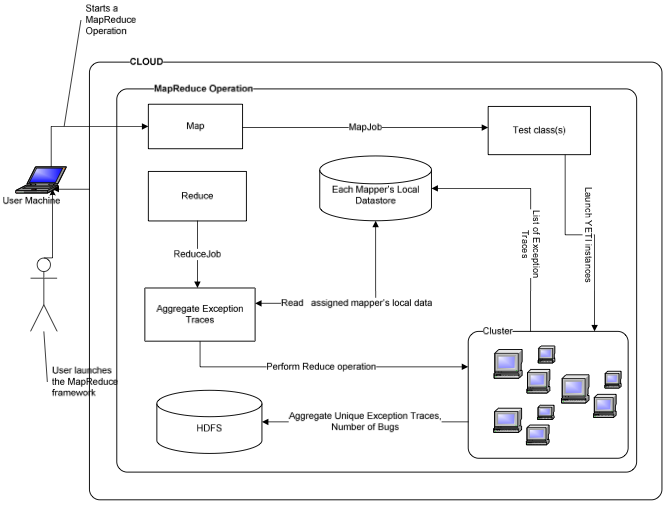
\includegraphics[width=\columnwidth]{images/YetiCloud.png}
\end{center}
\caption{YETI cloud architecture.}\label{fig:architecture}
\end{figure}


\subsection{Architecture of the cloud implementation}

As figure~\ref{fig:architecture} shows, the main architecture of YETI on the cloud 
relies on Hadoop, Apache's implementation of Google's map/reduce framework. 

The main idea is that we use a very simple approach where testing jobs 
are described by calls to YETI stored in normal text files by the user, that will each launch YETI in standalone mode. 
Commands from within each file are then mapped to different machines in the cloud. 

After setting up the map/reduce cluster. These text files and YETI (bundled as a jar file) are then uploaded to the 
distributed file system (DFS) on the map/reduce cluster master, which then launches individual testing machines 
for each text file executing the commands contained within the file in the order they appear.

At the end of the testing session, all exception traces are written back to the DFS during reduce step, which can then be downloaded to the 
user machine and made available to the software tester for evaluation.


\subsection{Evaluation}

We only ran preliminary evaluations.

We evaluated our approach using the Amazon Elastic Computing Cloud (EC2) \footnote{http://aws.amazon.com/ec2/}.
We performed 5 jobs of 20-minutes each (a total testing time of 100 minutes) in less 
than 21 minutes, outputting comparable results with YETI's standalone execution. 
Test cases all tested classes from \texttt{java.lang}.
The number of faults found in each tested class in the distributed mode were the same as those found during standalone execution of YETI. 

By using the cloud we clearly improved the performances of YETI and reduce the testing time by 
employing more machines and distributing the jobs. 
Distributing YETI over the cloud requires uploading the files containing typical YETI calls for launching YETI in standalone mode(multiple 
YETI calls can be placed in a file resulting in the same machine testing several programs or the same program with potentially specific options/strategies for each machine), and 
YETI itself (bundled as a Jar along with the classes to be tested). Setting up a Hadoop cluster on EC2  and uploading all the required files to the 
MapReduce Master then takes under a few minutes. However, setting up the EC2 cluster for the first time might 
take some  extra time (up to 10 minutes in our tests), but subsequent testing sessions require less than a few minutes to start. 
The execution can be performed on a locally set up Hadoop cluster as well. While we did not run experiments with 
more open security models, YETI jobs were run on one-shot Ubuntu virtual machines, which solves
the potential security issues for random testing.

\section{Future Work}\label{sec:future}

While this first experiment with YETI on the cloud was quite 
conclusive, there are many areas that we would like to improve 
in the future. In the next paragraphs, we explain some of these 
areas and what in our opinion we would need to do.

\paragraph{Define automated mappings for jobs}
It is still unclear what the best mapping for testing sessions would be for large 
amount of classes. So far, experiments have shown that testing classes
independently is not the best way to uncover faults. In particular, 
testing two classes that are used together (such as \texttt{String} and 
\texttt{StringBuilder}) uncovers faults that are not uncovered when tested 
independently. Grey-box testing might help in finding out which code is dependent 
on each other and would lead to better understanding of this phenomenon to make
the best mappings for testing sessions.

\paragraph{Define adequacy criteria for distributed random testing sessions}
In all tests that were performed it seems that the testing sessions
achieve a plateau if parameters of the testing session are unchanged. 
Being able to detect such plateaus would lead to stopping the testing sessions
when YETI does not have high chances to discover further faults. It could then
lead to a better way of mapping jobs on a low number of nodes.


\paragraph{Testing programs working over the cloud}
One of the issues with programs working on the cloud is that testing such 
programs requires to run tools that are themselves running on the cloud.
YETI could be one of these testing tools.


\paragraph{Real-time feedback on the distributed testing sessions}
One of the most valuable aspects of YETI is its graphical user interface~\cite{OriolTassis2010} 
which shows information about the testing session in real-time. The 
map/reduce middleware does not however allows for sending results in real-time
back to the master. This implies that a YETI on the cloud would benefit from a more 
flexible middleware such as Multicast Objects~\cite{mobjectsTR}.

\section{Related Work}\label{sec:rw}
Distributing software testing over multiple computers has received very little attention in the research community. Starkloff~\cite{stark} presents the general advantages of parallelizing software testing systems and how to achieve parallelism by distributing execution. 

Lastovetsky and Alexey~\cite{lasto} present a case for testing of a distributed programming system where serial execution of a regression test suite would on the average take at least 90 hours per bug detected, whereas Parallelizing the execution on a number of local UNIX computers resulted in a speed up of up to 7.7 on two 4-processor workstations, which meant the test suite could be run multiple times in a single day.

Further work resulted in tools like Joshua ~\cite{Kap}, and GridUnit~\cite{Duarte1, Duarte2, Duarte3}. 
Joshua uses Jini for distributing the execution of a regression test suite across a number of CPUs and 
writes the results back to a centralized repository, whereas GridUnit employs a computational Grid to speed up the testing process. 
A single master distributes test cases for execution across machines in a Grid and then waits for the results.
Both Joshua and GridUnit extend the JUnit testing framework. Using the same principles, Yao \textit{et al.}~\cite{yao} present the implementation of a grid-based unit testing framework and present some preliminary results based on simulation. 
The framework  differs from Joshua and GridUnit in its support for NUnit and dbUnit apart from JUnit, extending its support for C\# and database-driven projects.

Some of the limitations of such approaches, however, include the requirement that a test case be manually created beforehand, and their execution on either a local LAN or a Grid. A LAN has limited number of machines whereas, in a Grid, nodes might have different computational capacities varying from supercomputers to a low-end personal computer~\cite{yao}. This would seriously impact the performance 
of some test cases and work would have to be assigned according to the workers capacity. 

The only approach that is somewhat similiar to our implementatin for distributing execution is outlined in ~\cite{parveen}, where a prototype distributed execution framework for 
JUnit test cases called HadoopUnit is presented. They also use the MapReduce primitives for distributing test cases. Before execution can begin, an Ant task is run 
to produce input for the map function from uploaded files and stores them in a file to be later read by the Mapper. The Reducer then collects the test case results from each Mapper 
and outpputs them to a file on the DFS. A speed of 30x in execution time is reported on a 150-node cluster. 
However, HadoopUnit too only supports execution of JUnit test cases and requires them be created manually beforehand. 

YETI creates test cases on the fly, executes them against the target code and reports bugs. The use of a computational Cloud by YETI resolves the issues outlined above, 
since the test cases are created automatically, each node has the same processing power and new nodes can be added dynamically, if more processing power is required. 




\section{Limitations and Future Work}\label{sec:fut}

The approach currently has a few limitations:
\begin{itemize}
\item The socket communication can mess up with special characters used in exception traces. As we previously mentioned special characters might interfere with the regular process of the socket communication because it is text-based. It is likely that another format might be better for such communications. This will be investigated in the future.
\item There is no way of stopping infinite loops in the .NET binding. This is a serious limitation for the .NET binding at the moment as it is not possible to test some classes due to that limitation. A clean implementation is however much more difficult to realize, but we are planning to do it in the near future.
\item There is no restart of the system after the .NET part crashed. Currently, if the .NET part crashes, we do not restart the program. This is a limitation we need to overcome in order to test realistically the system libraries.
\item It is time-consuming to interpret failures as there is no parsing of the textual documentation.
Such a parsing is going to be necessary if we want to provide a significant support for .NET users.
It would also benefit other languages users (even Java) and make the interpretation of the testing much more reliable. It is however a challenging problem as documentation is typically informally written.
\end{itemize}

The efficiency of the socket-based communication also made clear that 
using socket-based communication between the program under test and the 
testing infrastructure was a viable alternative (100\% overhead only). 
This means that even in the Java biding it could be interesting to use 
such an approach for testing classes that may quit the program. While this 
is seldom the case for libraries, this might be useful for end-user classes.
\section{Conclusions}\label{sec:conc}
This article presents YETI, a new tool to run automated random testing 
sessions of Java programs. YETI runs at a very high speed -- around $10^{6}$ calls per 
minute on fast code -- and provides a graphical user interface that allows test engineers to
diagnose the testing process while testing. Test engineers are then able to 
change parameters and types used in the testing session while it proceeds.
To validate our approach we used YETI on \texttt{java.lang} and on a package
of a popular open source library. YETI found 45 faults in 
\texttt{java.lang} and 120 in the open source library.

Future work will further focus on visualising better the result of the testing process 
by presenting intuitive representations of the failure domains.


%\section{Introduction}
% The very first letter is a 2 line initial drop letter followed
% by the rest of the first word in caps.
% 
% form to use if the first word consists of a single letter:
% \IEEEPARstart{A}{demo} file is ....
% 
% form to use if you need the single drop letter followed by
% normal text (unknown if ever used by IEEE):
% \IEEEPARstart{A}{}demo file is ....
% 
% Some journals put the first two words in caps:
% \IEEEPARstart{T}{his demo} file is ....
% 
% Here we have the typical use of a "T" for an initial drop letter
% and "HIS" in caps to complete the first word.
%\IEEEPARstart{T}{his} demo file is intended to serve as a ``starter file''
%for IEEE journal papers produced under \LaTeX\ using
%IEEEtran.cls version 1.7 and later.
% You must have at least 2 lines in the paragraph with the drop letter
% (should never be an issue)
%I wish you the best of success.

%\hfill mds
% 
%\hfill January 11, 2007

%\subsection{Subsection Heading Here}
%Subsection text here.

% needed in second column of first page if using \IEEEpubid
%\IEEEpubidadjcol

%\subsubsection{Subsubsection Heading Here}
%Subsubsection text here.


% An example of a floating figure using the graphicx package.
% Note that \label must occur AFTER (or within) \caption.
% For figures, \caption should occur after the \includegraphics.
% Note that IEEEtran v1.7 and later has special internal code that
% is designed to preserve the operation of \label within \caption
% even when the captionsoff option is in effect. However, because
% of issues like this, it may be the safest practice to put all your
% \label just after \caption rather than within \caption{}.
%
% Reminder: the "draftcls" or "draftclsnofoot", not "draft", class
% option should be used if it is desired that the figures are to be
% displayed while in draft mode.
%
%\begin{figure}[!t]
%\centering
%\includegraphics[width=2.5in]{myfigure}
% where an .eps filename suffix will be assumed under latex, 
% and a .pdf suffix will be assumed for pdflatex; or what has been declared
% via \DeclareGraphicsExtensions.
%\caption{Simulation Results}
%\label{fig_sim}
%\end{figure}

% Note that IEEE typically puts floats only at the top, even when this
% results in a large percentage of a column being occupied by floats.


% An example of a double column floating figure using two subfigures.
% (The subfig.sty package must be loaded for this to work.)
% The subfigure \label commands are set within each subfloat command, the
% \label for the overall figure must come after \caption.
% \hfil must be used as a separator to get equal spacing.
% The subfigure.sty package works much the same way, except \subfigure is
% used instead of \subfloat.
%
%\begin{figure*}[!t]
%\centerline{\subfloat[Case I]\includegraphics[width=2.5in]{subfigcase1}%
%\label{fig_first_case}}
%\hfil
%\subfloat[Case II]{\includegraphics[width=2.5in]{subfigcase2}%
%\label{fig_second_case}}}
%\caption{Simulation results}
%\label{fig_sim}
%\end{figure*}
%
% Note that often IEEE papers with subfigures do not employ subfigure
% captions (using the optional argument to \subfloat), but instead will
% reference/describe all of them (a), (b), etc., within the main caption.


% An example of a floating table. Note that, for IEEE style tables, the 
% \caption command should come BEFORE the table. Table text will default to
% \footnotesize as IEEE normally uses this smaller font for tables.
% The \label must come after \caption as always.
%
%\begin{table}[!t]
%% increase table row spacing, adjust to taste
%\renewcommand{\arraystretch}{1.3}
% if using array.sty, it might be a good idea to tweak the value of
% \extrarowheight as needed to properly center the text within the cells
%\caption{An Example of a Table}
%\label{table_example}
%\centering
%% Some packages, such as MDW tools, offer better commands for making tables
%% than the plain LaTeX2e tabular which is used here.
%\begin{tabular}{|c||c|}
%\hline
%One & Two\\
%\hline
%Three & Four\\
%\hline
%\end{tabular}
%\end{table}


% Note that IEEE does not put floats in the very first column - or typically
% anywhere on the first page for that matter. Also, in-text middle ("here")
% positioning is not used. Most IEEE journals use top floats exclusively.
% Note that, LaTeX2e, unlike IEEE journals, places footnotes above bottom
% floats. This can be corrected via the \fnbelowfloat command of the
% stfloats package.


%
%\section{Conclusion}
%The conclusion goes here.





% if have a single appendix:
%\appendix[Proof of the Zonklar Equations]
% or
%\appendix  % for no appendix heading
% do not use \section anymore after \appendix, only \section*
% is possibly needed

% use appendices with more than one appendix
% then use \section to start each appendix
% you must declare a \section before using any
% \subsection or using \label (\appendices by itself
% starts a section numbered zero.)
%


%\appendices
%\section{Proof of the First Zonklar Equation}
%Appendix one text goes here.

%% you can choose not to have a title for an appendix
%% if you want by leaving the argument blank
%\section{}
%Appendix two text goes here.

%\section*{Appendix}
\begin{verbatim}
using System;
using System.Collections.Generic;
using System.Diagnostics.Contracts;

namespace YetiTestAssembly1
{
    class Object1
    {
        public double doubleAttr1;
        public String s1;

        public Object1()
        {
            doubleAttr1 = 10.00;
            s1 = "";
        }

        public int methodReturnInt1(int r, int t)
        {
            Contract.Ensures(Contract.Result<int>() != 0);
            r = t;
            return r;
        }

        public void setDoubleAttr1(double d)
        {
            Contract.Ensures(d > 10.5);
            doubleAttr1 = d;
        }

        public String returnStringValue1()
        {
            return "A test String Object1";
        }

        public float methodForFloat1(Object1 ob, char c, long l)
        {
            Contract.Requires(ob != null && c != 'm');
            Contract.Ensures(l > 100);
            float f = (Single)l;
            return f;
        }

        public static void addingTwoInts1(int a, int b)
        {
            a = a + b;
        }

        public char returnCharValue1()
        {
            return 'c';
        }

        static void Main(string[] args)
        {
            Console.WriteLine("Starting Object1 Main method");
        }
    }
}
using System;
using System.Collections.Generic;
using System.Diagnostics.Contracts;

namespace YetiTestAssembly2
{
    class Object2
    {
        public double doubleAttr2;
        public Object2 ob2;

        public Object2()
        {
            doubleAttr2 = 55.22;
            ob2 = null;
        }

        public int methodReturnInt2(int r, int t)
        {
            Contract.Ensures(Contract.Result<int>() > 5);
            r = t;
            return r;
        }

        public void setOb2Attr(Object2 d)
        {
            Contract.Ensures(d !=null);
            ob2 = d;
        }

        public String returnStringValue2()
        {
            return "A test String Object2 fffff///***";
        }

        public float methodForFloat2(double ob, int l)
        {
            Contract.Requires(ob != 0.0);
            Contract.Ensures(Contract.Result<float>() != 0);
            float f = (Single)(l*ob);
            return f;
        }

        public static void addingTwoShorts2(short a, short b)
        {
            int h = a + b;           
        }

        public char returnCharValue2()
        {
            return 'U';
        }

        public Object2 genOb2()
        {
            return new Object2();
        }

        static void Main(string[] args)
        {
            Console.WriteLine("Starting Object2 Main method");
        }
    }
}
using System;
using System.Collections.Generic;
using System.Diagnostics.Contracts;
namespace YetiTestAssembly3
{
    class Object3
    {
        public double doubleAttr3;
        public int intAttr3;
        public Object3 ob3;

        public Object3()
        {
            doubleAttr3 = 333.333;
            intAttr3 = 1;
            ob3 = null;
        }

        public Object3(int t, double d, Object3 o)
        {
            doubleAttr3 = d;
            intAttr3 = t;
            ob3 = o;
        }

        public static int methodReturnInt3(int r, int t)
        {
            Contract.Requires(t != 4);
            Contract.Ensures(Contract.Result<int>() > 1);
            r = t;
            return r;
        }

        public void setOb3Attr(Object3 d, char c, String s)
        {
            Contract.Ensures(d !=null && c!='m');
            ob3 = d;
        }

        public String returnStringValue3()
        {
            return "ggg333nnn";
        }

        public float methodForFloat3(double ob, int l)
        {
            Contract.Requires(ob != 0.0);
            Contract.Ensures(Contract.Result<float>() != 100);
            float f = (Single)(l*ob);
            return f;
        }

        public static void dividingTwoShorts3(short a, short b)
        {
            Contract.Assert(b!=0);
            short h;
            h = Convert.ToInt16(a/b);
        }

        public char returnCharValue3()
        {
            return 'Y';
        }

        public Object3 genOb3()
        {
            return new Object3();
        }

        static void Main(string[] args)
        {
            Console.WriteLine("Starting Object3 Main method");
        }
    }
}
\end{verbatim}

%
%% use section* for acknowledgement
%\section*{Acknowledgment}

%
%The authors would like to thank...

%
% Can use something like this to put references on a page
% by themselves when using endfloat and the captionsoff option.
\ifCLASSOPTIONcaptionsoff
  \newpage
\fi



% trigger a \newpage just before the given reference
% number - used to balance the columns on the last page
% adjust value as needed - may need to be readjusted if
% the document is modified later
%\IEEEtriggeratref{8}
% The "triggered" command can be changed if desired:
%\IEEEtriggercmd{\enlargethispage{-5in}}

% references section

% can use a bibliography generated by BibTeX as a .bbl file
% BibTeX documentation can be easily obtained at:
% http://www.ctan.org/tex-archive/biblio/bibtex/contrib/doc/
% The IEEEtran BibTeX style support page is at:
% http://www.michaelshell.org/tex/ieeetran/bibtex/
\bibliographystyle{IEEEtran}
% argument is your BibTeX string definitions and bibliography database(s)
\bibliography{Biblio}
%
% <OR> manually copy in the resultant .bbl file
% set second argument of \begin to the number of references
% (used to reserve space for the reference number labels box)
%\begin{thebibliography}{1}

%\bibitem{IEEEhowto:kopka}
%H.~Kopka and P.~W. Daly, \emph{A Guide to \LaTeX}, 3rd~ed.\hskip 1em plus
%  0.5em minus 0.4em\relax Harlow, England: Addison-Wesley, 1999.

%\end{thebibliography}



% biography section
% 
% If you have an EPS/PDF photo (graphicx package needed) extra braces are
% needed around the contents of the optional argument to biography to prevent
% the LaTeX parser from getting confused when it sees the complicated
% \includegraphics command within an optional argument. (You could create
% your own custom macro containing the \includegraphics command to make things
% simpler here.)
%\begin{biography}[{\includegraphics[width=1in,height=1.25in,clip,keepaspectratio]{mshell}}]{Michael Shell}
% or if you just want to reserve a space for a photo:

\begin{IEEEbiography}{Manuel Oriol}
Biography text here.
\end{IEEEbiography}

% if you will not have a photo at all:
\begin{IEEEbiographynophoto}{Sotirios Tassis}
Biography text here.
\end{IEEEbiographynophoto}

% insert where needed to balance the two columns on the last page with
% biographies
%\newpage

%\begin{IEEEbiographynophoto}{Jane Doe}
%Biography text here.
%\end{IEEEbiographynophoto}

% You can push biographies down or up by placing
% a \vfill before or after them. The appropriate
% use of \vfill depends on what kind of text is
% on the last page and whether or not the columns
% are being equalized.

%\vfill

% Can be used to pull up biographies so that the bottom of the last one
% is flush with the other column.
%\enlargethispage{-5in}



% that's all folks
\end{document}


